% Kapitel Ergebnisse der Hausarbeit

\subsection{Hauptbefunde}
Hier die wichtigsten Schätzergebnisse in zusammengefasster Form darstellen.
% SLOT E1 — Hauptbefunde H1 (2-3 eigene Saetze + Verweis auf Anhangstabellen)
% NOTIZ (Zahlen aus results/phase_b/tables/phase_b_modellvergleich.csv und
% phase_b_hypothesen_robustheit.csv — vor Abgabe gegen CSV pruefen):
%   H1 Basismodell (Laender-FE, nur nrquarterssmpl): unsc3 = -0,45 (SE 1,85), p = 0,81, n = 514.
%   H1 Vollmodell (Laender-FE, DSV-Kontrollen): unsc3 = +0,14 (SE 2,82), p = 0,96, n = 282.
%   H1 Hauptmodell (Laender- und Jahres-FE): unsc3 = -0,93 (SE 1,92), p = 0,63, n = 281, davon 24 unsc3-Jahre.
% Fazit H1: kein signifikanter Effekt im modernen Zeitraum (1992-2023),
% anders als im Originalzeitraum (dort ca. 30 Prozent weniger Konditionen).

% SLOT E2 — Hauptbefunde H2/H4 (2-3 eigene Saetze)
% NOTIZ (Zahlen aus phase_b_hypothesen_robustheit.csv,
% phase_b_h2_leave_one_country_out.csv, phase_b_h4_leave_one_country_out.csv):
%   H2 Hauptmodell: unsc3:resource_dep = -0,11 (SE 0,10), p = 0,29, n = 212.
%   H2 Robustheit Fuel-Exporte: -0,22, p = 0,024 — EINZIGE signifikante Spezifikation.
%   H2 Robustheit Mineral-Exporte: +0,01, p = 0,91. Placebo (ExportGDP): -0,12, p = 0,37.
%   H4 explorativ (s. Tab. 7, phase_b_h4_ergebnisse.tex): Interaktion -1,93e-06 (SE 4,96e-04), p = 0,997, n = 212; Robustheiten Fuel/Mineral/Kreditbestand/winsor alle n.s.; Zeitfenster 1992-2008 p = 0,307, 2009-2023 p = 0,706.
%   Leave-one-out (H2): ohne PER -0,19, ohne GAB -0,04 → die Interaktion
%   haengt an einzelnen Laendern (Instabilitaet erwaehnen).
%   H2-Zeitfenster: 1992-2008 +0,27 (p = 0,012, signifikant POSITIV),
%   2009-2023 -0,38 (p = 0,072) — die Interaktionsrichtung DREHT
%   zwischen den Fenstern; in der H2-Interpretation sauber einordnen
%   (Haupttest: Gesamtzeitraum; Fenster sind Robustheit).
%   H1 Poisson-FE (S2-Analog): -0,043, p = 0,78 — Semi-Elastizitaet
%   ca. 4 Prozent weniger Bedingungen pro Quartal, nicht signifikant.
% ACHTUNG: Der bestehende Satz "kein stabiler signifikanter Effekt" im
% Interpretation-Absatz unten muss die Fuel-Export-Ausnahme (p = 0,024)
% und die Leave-one-out-Sensitivitaet sauber einordnen.


\subsection{Interpretation}
Interpretation der Richtung, Stärke und Bedeutung der Effekte in der Sprache der Forschung.
% SLOT E3 — Sprechweise: Punktschaetzer vs. Unsicherheit (kein eigener
% Absatz noetig; die Unterscheidung nur in den Interpretations-Saetzen
% anwenden, danach diesen Marker entfernen)
% NOTIZ (Begriffsklaerung als Schreibhilfe — NICHT als Lehrbuch-Definition
% in die Arbeit uebernehmen):
% - Punktschaetzer = der einzelne Zahlenwert des Koeffizienten, der
%   "Rat" des Modells: z.B. H2-Interaktion -0,11.
% - Standardfehler = typische Unsicherheit des Rats (hier 0,10).
% - p-Wert = Wahrscheinlichkeit, mindestens ein so grosses
%   Punktschaetzer-Ergebnis zu sehen, wenn der wahre Wert null waere
%   (hier 0,29).
% Formulierungsregeln fuer die eigenen Saetze:
% - "Der Punktschaetzer zeigt Richtung X" ist KEIN Beweis fuer X.
% - Insignifikant heisst "nicht von null unterscheidbar", NICHT
%   "belegt null" (vgl. Zeitfenster 2002-2008: -1,86 bei p = 0,52).
% - Musteranwendung Differenztest: "Die Punktschaetzer sprechen fuer
%   eine Abschwaechung des Effekts nach 2002 (+2,5), der formale Test
%   verfehlt jedoch die Signifikanz (p = 0,36)."


In den Robustness-Checks zeigt sich kein stabiler signifikanter Effekt von UNSC-Mitgliedschaft, Ressourcenabhängigkeit 
oder ihrer Interaktion auf die IMF-Konditionalität. 
Die Ergebnisse sind insgesamt inkonsistent und sprechen eher gegen einen robusten Moderationseffekt.

Das heißt: Die Daten liefern in diesem Spezifikationsrahmen keine belastbare Evidenz für einen signifikanten Haupteffekt 
oder einen signifikanten gemeinsamen Effekt.
% ----------------------------------------------------------------------
% INTERPRETATION H1-H3 — eigener Entwurf (2026-10-05), faktisch
% korrigiert. Verbleibende Pruefpunkte als TODO am jeweiligen Block.
% ----------------------------------------------------------------------
Die Zerlegung des Originalzeitraums zeigt, dass der publizierte Effekt zeitlich von den 1990er-Jahren getragen wird: In den Punktschätzern zeichnet sich bereits Anfang und Mitte der 2000er, begleitet vom Rückgang der Nachfrage nach IMF-Krediten \parencite[545]{KentikelenisIMFConditionalityDevelopment2016}, eine Abschwächung ab; der formale Differenztest verfehlt allerdings wegen der kleinen Stichprobe die Signifikanz. Mit dem über den Originalzeitraum hinaus bis 2023 erweiterten Panel lässt sich dieser Trend weiter beobachten. Der Nullbefund ist dabei kein Artefakt der IMF-Inaktivität: Auch in der Phase massiver Nachkrisen-Kreditvergabe ab 2009 zeigt sich kein UNSC-Effekt. Als Deutungsangebot bietet sich an, dass die Einflusskauf-Logik an die geopolitische Konstellation der 1990er gebunden war und nach deren Ende an Bedeutung verlor.
% TODO (H1): Zeitfenster-Tabelle (original_replication_zeitfenster) fehlt
% bisher im Anhang — entweder aufnehmen oder die Zerlegung hier nur
% verbal belegen (1992-2001: -4,65; 2002-2008: -1,86).
% TODO (H1): Momani & Helleiner 2007 nicht in literatur.bib — als
% Sekundaerzitat ueber Kentikelenis et al. belassen oder nachtragen.

Die Behauptung, die Rohstoffabhängigkeit moderiere den UNSC-Effekt derart, dass sich dieser in rohstoffabhängigeren Ländern stärker zugunsten der UNSC-Mitglieder — in noch weniger Bedingungen — ausprägt, lässt sich nicht bestätigen. Nur in einer Spezifikation, die Rohstoffabhängigkeit ausschließlich über die Erdöl-Exportquote misst, zeigt sich eine signifikante Moderation; die Mineral- und Placebo-Varianten bleiben null, und die Leave-one-out-Analyse zeigt, dass die Hauptinteraktion von einzelnen Ländern abhängt. Ein Allgemeineffekt lässt sich von der Erdöl-Spezifikation nicht ableiten.
% TODO (H2): Tabellenverweise ergaenzen (Anhang: H2-Ergebnisse,
% H2-Modellvergleich, Robustheitstabelle) und gegen das PDF pruefen.

Die Länder im untersten Quartil der Konditionalität (2,0 bis 7,2 Bedingungen pro Quartal) sind in Bezug auf die Rohstoffabhängigkeit heterogen verteilt: von Äthiopien (0,8\,\%) und Mali (0,6\,\%) über Kenia (12,7\,\%) bis Peru (43,6\,\%); selbst der Irak (98,6\,\%) liegt mit 7,8 Bedingungen nur marginal über der Quartilsgrenze. Unter den Ländern mit den höchsten Konditionalitäten (75. Perzentil bis Maximum, 12,5 bis 40,5 Bedingungen) reicht die Spanne von Irland (31,4 Bedingungen bei 2,3\,\% Rohstoffabhängigkeit) über Griechenland (17,7 bei 40,4\,\%) bis Angola (20,3 bei 99,3\,\%); Portugal markiert mit 40,5 Bedingungen bei 10,4\,\% das Maximum. Aus der Rohstoffabhängigkeit allein lassen sich daher keine systematischen Zusammenhänge mit der Höhe der Bedingungen pro Quartal ableiten. Im Innerhalb-Länder-Vergleich der UNSC-Länder (die vollständigen Länderprofile sind als Reproduktionsmaterial im Repository der Arbeit einsehbar) zeigt sich dieselbe Heterogenität anhand der Differenzen zwischen den Bedingungs-Mittelwerten in UNSC-Jahren und Nicht-UNSC-Jahren: Unter den rohstoffabhängigeren UNSC-Ländern mischen sich positive Lücken (Niger +14,7, Ruanda +16,4, Ägypten +7,2, Mosambik +3,4) und negative (Gabun -4,3, Guinea -9,9). Die Lückenfolge folgt somit nicht der Rohstoffabhängigkeit — konsistent mit dem H2-Nullbefund.
% TODO (H3): Die Quartils-/Perzentilwerte stammen aus den
% Explorationstabellen (konditionalitaet_perzentile etc.), die nicht
% Teil der Hausarbeit sind — fuer die Abgabe entweder als eigene
% Berechnung im Anhang dokumentieren oder die Formulierung vollstaendig
% auf Tabelle 6 stuetzen.



\begin{figure}[h]
\centering
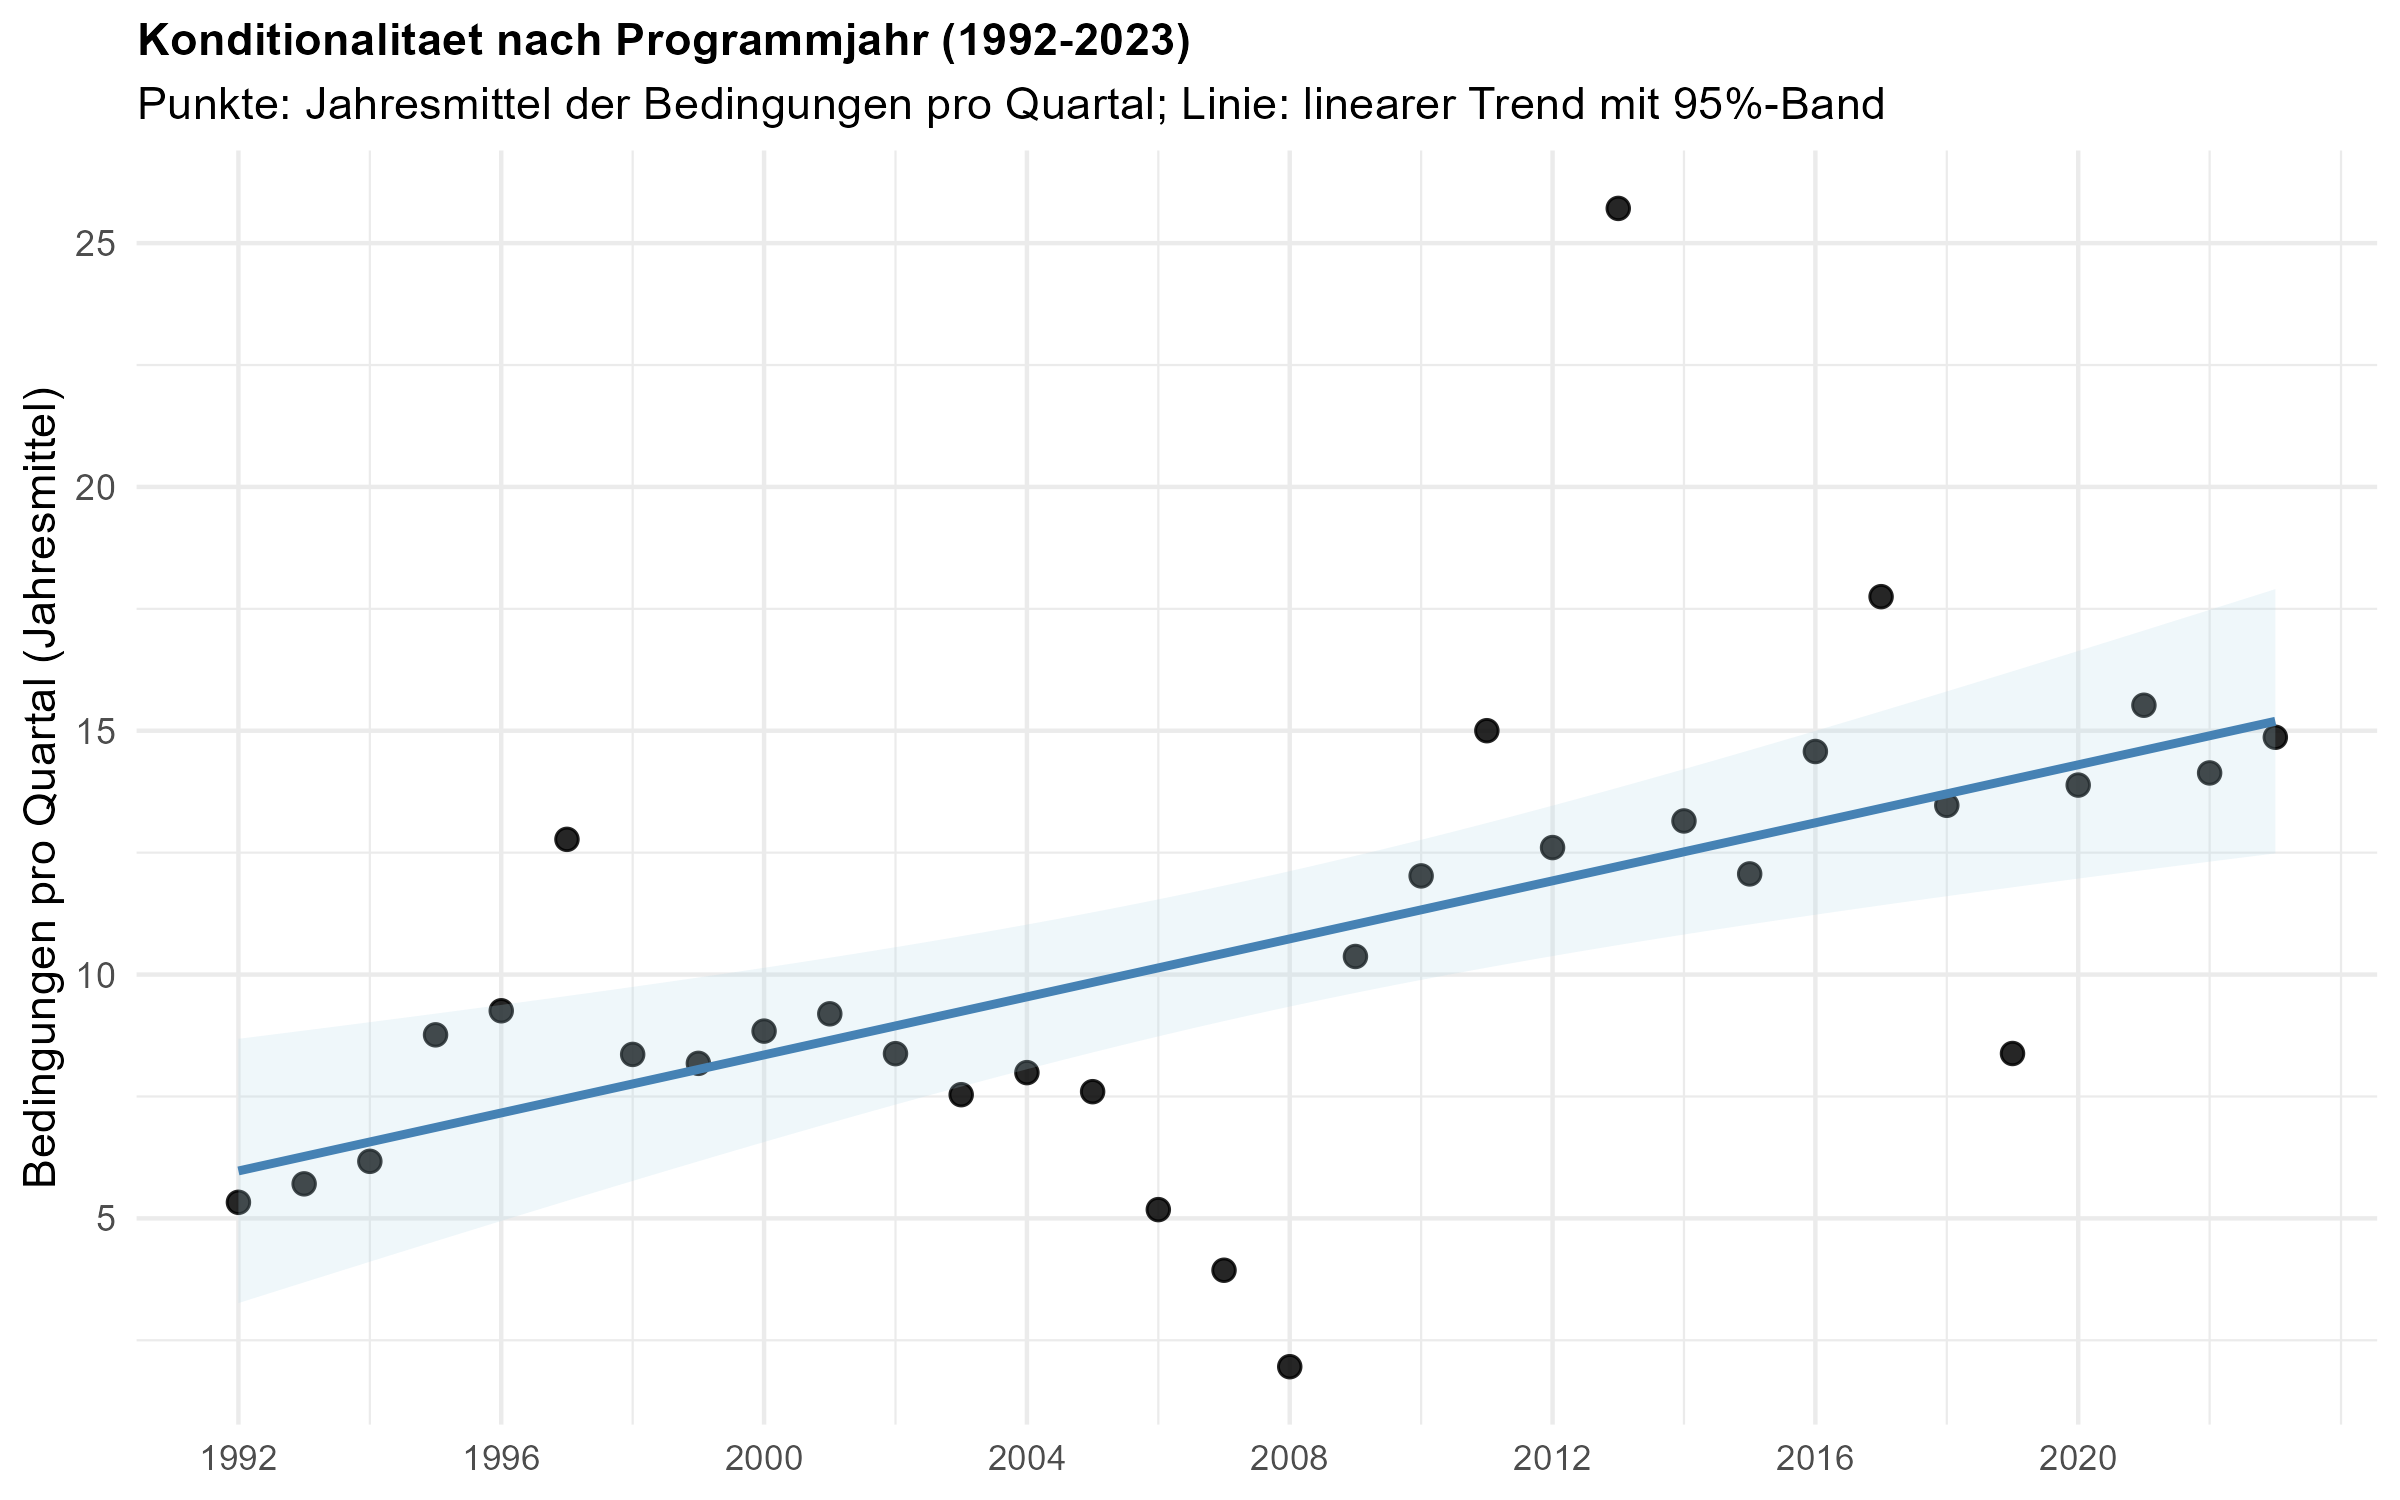
\includegraphics[width=0.85\textwidth]{figures/phase_b/konditionalitaet_jahresreihe.png}
\caption{Bedingungen pro Quartal nach Programmjahr, 1992--2023 (Punkte: Jahresmittel; Linie: linearer Trend mit 95-Prozent-Band). Deskriptive Kontextdarstellung; die Jahres-Fixed-Effects der Modelle absorbieren dieses Niveau.}
\label{fig:konditionalitaet-jahresreihe}
\end{figure}

% SLOT E4 — Verweis-Satz auf die Abbildung (1-2 eigene Saetze)
% Behauptung: Die Abbildung zeigt den Epochenwechsel: historisches
% Nachfragetief 2008 (nur 6 Programmjahre, 2,0 Bedingungen/Quartal),
% danach Anstieg auf rund das Doppelte des 1990er-Niveaus (Spitze 2013).
% Verknuepfen mit der H1-Einordnung (SLOT E1) und dem IMF-Rueckkehr-
% Argument (SLOT D1 in diskussion.tex, Kentikelenis et al. S. 545).
% Daten: results/phase_b/exploration/konditionalitaet_jahresreihe.csv;
% Skript: code/phase_b/analysis/phase_b_ressourcen_exploration.R,
% Sektionen F (Daten) und G (Abbildung).

% TODO vor Abgabe: Diese Anmerkung final formulieren oder als
% Robustheits-/Einordnungsabsatz in die Ergebnisse/Diskussion übernehmen.
\paragraph{Explorative Zusatzanalyse: Komposition der Bedingungen}
Die Komposition der Bedingungen wird rein deskriptiv ausgewertet (Skript
\texttt{code/phase\_b/analysis/phase\_b\_komposition\_exploration.R}; Output
\texttt{results/phase\_b/exploration/komposition\_ressourcen\_quartile.csv}
sowie \texttt{.../komposition\_ressourcen\_quartile\_unsc3.csv}). Stichprobe:
396 Land-Jahre mit \texttt{resource\_dep} (1992--2023); Quartilsgrenzen der
Rohstoffabhängigkeit bei 3{,}8 / 11{,}8 / 35{,}3 Prozent der Warenexporte.

\begin{table}[h]
\centering
\begin{tabular}{lrrr}
\hline
Quartil & Bedingungen & Rohstoff-Anteil (gew.) & Stabilitäts-Anteil \\
\hline
Q4 (hoch) & 12.471 & 3{,}7 \% & 28{,}9 \% \\
Q3 & 12.297 & 4{,}1 \% & 29{,}4 \% \\
Q2 & 12.722 & 2{,}3 \% & 26{,}6 \% \\
Q1 (niedrig) & 10.858 & 2{,}3 \% & 26{,}0 \% \\
\hline
\end{tabular}
\caption{Anteil rohstoff- bzw. stabilitätsklassifizierter Bedingungen nach Quartilen der Rohstoffexportabhängigkeit (deskriptiv, gewichtete Anteile)}
\end{table}

Deskriptiv zeigt sich der erwartbare Gradient: In der oberen Hälfte der
Rohstoffabhängigkeit liegt der Anteil explizit extraktivbezogener Bedingungen
fast doppelt so hoch wie unten (4{,}1 bzw. 3{,}7 Prozent gegen 2{,}3 Prozent),
während der Stabilitätsanteil weitgehend flach bleibt. Im Quartil-$\times$-UNSC-Schnitt
(sehr kleine UNSC-Zellen, 6--10 Fälle je Quartil) liegt der Rohstoffanteil bei
UNSC-Jahren durchweg niedriger als bei Nicht-UNSC-Jahren — ein Zahlenmuster,
das zur H2-Richtung passt, aber wegen Zellgröße und Klassifikationsunsicherheit
nur als Beschreibung taugt. Die Einschränkungen (417 historische Zeilen ohne
Beschreibungstext werden als nicht rohstoffbezogen kodiert; keine Inferenz)
dokumentiert das Skript mit.

% ----------------------------------------------------------------------
% INTERPRETATION H4 — eigener Entwurf (2026-10-05), faktisch korrigiert.
% ----------------------------------------------------------------------
H4 wurde aufgrund der Klassifikationsunsicherheit der selbst definierten Rohstoff- und Stabilitätsklassifikationen aus dem konfirmatorischen Pfad genommen; die Analyse der Bedingungsinhalte in Kombination mit der UNSC-Mitgliedschaft ist als rein explorativ zu verstehen. Die explorative Schätzung ergibt keine Moderation durch die UNSC-Mitgliedschaft: Die Veränderung über die gesamte Spannweite der Rohstoffabhängigkeit beträgt weniger als 0{,}02 Prozentpunkte, und in keiner Spezifikation zeigt sich ein Muster, das die Kompositionshypothese stützen würde. Abwegig ist der Rohstoff-Ansatz allerdings nicht: Über die Quartilstabelle (Tabelle 1) lässt sich zumindest deskriptiv eine plausible Korrelation der Klassifikation mit der Rohstoffabhängigkeit ablesen — ein Hinweis auf inhaltliche Validität. In der oberen Hälfte der Rohstoffabhängigkeit liegt der Anteil rohstoffbezogener Bedingungen deutlich höher als in der unteren, wobei der Gradient aus zwei Gründen leicht ausfällt: Der Absolutwert liegt selbst in Q3/Q4 nur bei 4{,}1 bzw. 3{,}7 Prozent, und der Anstieg verläuft nicht monoton, sondern verdoppelt sich nur im Übergang von der unteren zur oberen Hälfte. Relativ zum Niveau betrachtet ist das Muster dennoch spezifisch: Der Stabilitätsanteil schwankt um weniger als ein Zehntel seines Niveaus (26{,}0 bis 28{,}9 Prozent), während sich der Rohstoffanteil verdoppelt — die Verschiebung betrifft also gezielt den Rohstoff-Inhalt und ist keine bereichsübergreifende Dynamik. Kritisch ist anzumerken, dass der Gradient teilweise mechanisch sein kann, da Bedingungen mit Rohstoffbezug nur dort auftreten, wo ein Rohstoffsektor ökonomisch bedeutsam ist. Insgesamt bleibt die Kompositionshypothese damit ein Kandidat für eine Folgestudie mit belastbarerer Klassifikation.
% TODO (H4): Tabellenverweise (Tabelle 1, Tabelle 7) gegen das
% kompilierte PDF pruefen; ggf. \cref statt fester Nummern verwenden.
